\documentclass{article}
\usepackage[utf8]{inputenc}
\usepackage{tcolorbox}
\usepackage{algpseudocode}
\usepackage{algorithm}
\usepackage{hyperref}
\hypersetup{
    colorlinks=true,
    linkcolor=blue,
    filecolor=magenta,      
    urlcolor=cyan,
    pdftitle={Overleaf Example},
    pdfpagemode=FullScreen,
    }

\urlstyle{same}
\floatname{algorithm}{Algorithm}
\usepackage{listings}
\usepackage{xcolor}


\usepackage{graphicx, multicol, latexsym, amsmath, amssymb}
\usepackage{blindtext}
\usepackage{subfigure}
\usepackage{caption}
\usepackage{capt-of}
\usepackage{tabu}
\usepackage{hyperref}
\usepackage{booktabs}

\usepackage{array}
\newcolumntype{P}[1]{>{\centering\arraybackslash}p{#1}}

% Default fixed font does not support bold face
\DeclareFixedFont{\ttb}{T1}{txtt}{bx}{n}{10} % for bold
\DeclareFixedFont{\ttm}{T1}{txtt}{m}{n}{10}  % for normal

% Custom colors
\usepackage{color}
\definecolor{deepblue}{rgb}{0,0,0.5}
\definecolor{deepred}{rgb}{0.6,0,0}
\definecolor{deepgreen}{rgb}{0,0.5,0}

\usepackage{listings}

% Python style for highlighting
\newcommand\pythonstyle{\lstset{
language=Python,
basicstyle=\ttm,
morekeywords={self},              % Add keywords here
keywordstyle=\ttb\color{deepblue},
emph={MyClass,__init__},          % Custom highlighting
emphstyle=\ttb\color{deepred},    % Custom highlighting style
stringstyle=\color{deepgreen},
frame=tb,                         % Any extra options here
showstringspaces=false,
    breakatwhitespace=false,         
    breaklines=true,  
}}


% Python environment
\lstnewenvironment{python}[1][]
{
\pythonstyle
\lstset{#1}
}
{}

% Python for external files
\newcommand\pythonexternal[2][]{{
\pythonstyle
\lstinputlisting[#1]{#2}}}

% Python for inline
\newcommand\pythoninline[1]{{\pythonstyle\lstinline!#1!}}
 
\newcommand{\arraySpaceFive}[5]{%
\begin{center}%
\begin{tabular}{|c|c|c|c|c|}%
\hline #1 & #2 & #3 & #4 & #5 \\ \hline %
\end{tabular} %
\end{center} %
}

\newcommand{\arraySpaceFour}[4]{%
\begin{center}%
\begin{tabular}{|c|c|c|c|}%
\hline #1 & #2 & #3 & #4 \\ \hline %
\end{tabular} %
\end{center} %
}

\title{\LARGE \textbf{Nodal Analysis} Studio Report \\ \Small CG1111A Studio 3}

\author{Prannaya Gupta (B02)}

\begin{document}

\maketitle

\section{Activity 1}

\begin{figure}[htbp]
\centering
\subfigure[The Given Set-Up] {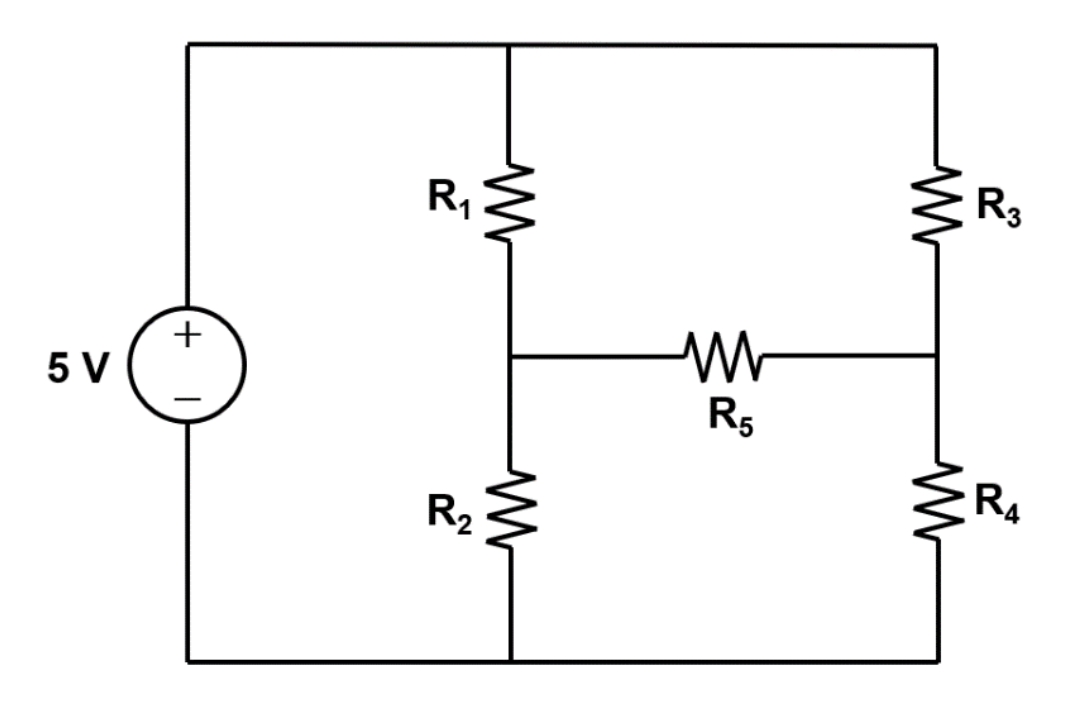
\includegraphics[width=0.5\textwidth]{images/setup.png}}\label{fig:setup}
\subfigure[Breadboard Used]{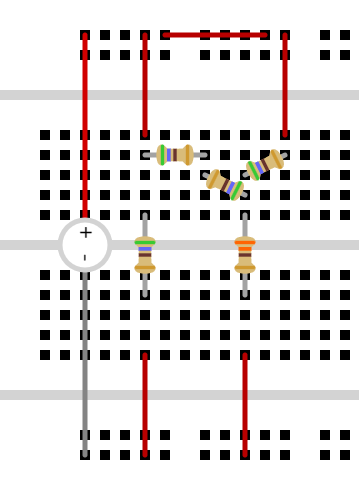
\includegraphics[width=0.25\textwidth]{images/breadboard.png}}\label{fig:breadboard}

\caption{Set-Up Planned} \label{fig:1}
\end{figure}

In this experiment, to utilise a Breadboard to its best usage under this system, we have designed it as shown in Figure \ref{fig:1}. \\

We know the individual resistances of each of these resistors (both Nominal and Measured via DMM), as shown in Table \ref{tab:resistances}.

\begin{table}[!h]
    \centering
    \begin{tabular}{|c|c|c|}
        \hline Resistor & Nominal Resistance ($\Omega$) & Measured Resistance ($\Omega$) \\
        \hline R_1 & 560 & 545 \\
        \hline R_2 & 560 & 546 \\
        \hline R_3 & 560 & 549 \\
        \hline R_4 & 330 & 324 \\
        \hline R_5 & 560 & 549 \\
        \hline
    \end{tabular}
    \caption{Table of Resistance Values}
    \label{tab:resistances}
\end{table}

We use nodal analysis to determine the relevant equations. We note that we denote $I_n$ as the current flowing through the resistor $R_n$.

\begin{figure}[h!]
    \centering
    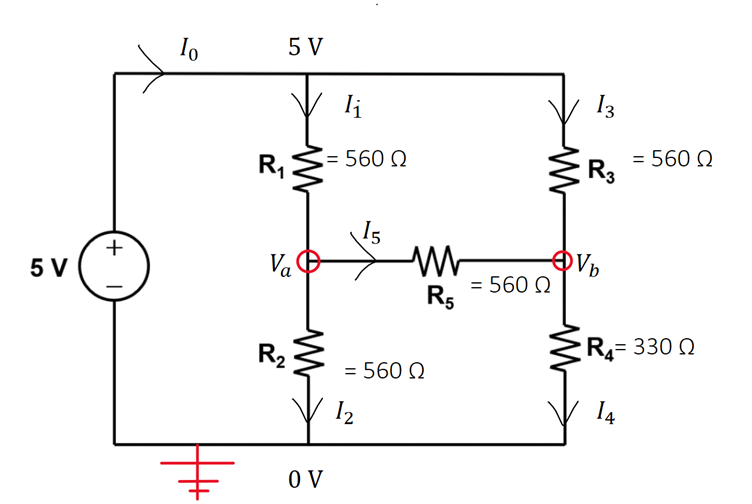
\includegraphics[width=\textwidth]{images/nodalAnalysis.png}
    \caption{Nodal Analysis performed on the Set-Up.}
    \label{fig:nodal}
\end{figure}


From here, we can use Kirchoff's Junction Law (KCL) to get the following equations:

\begin{align}
    \frac{5-V_a}{R_1} + \frac{V_b - V_a}{R_5} + \frac{0-V_a}{R_2} &= 0 \\
    \frac{5-V_b}{R_3} + \frac{V_a-V_b}{R_5} + \frac{0-V_b}{R_4} &= 0
\end{align}

We can simplify this to get the following equations:

\begin{align}
    \left(\frac{1}{R_1} + \frac{1}{R_5} + \frac{1}{R_2}\right) V_a - \frac{1}{R_5}V_b &= \frac{5}{R_1} \\
    \left(\frac{1}{R_3} + \frac{1}{R_5} + \frac{1}{R_4}\right) V_b - \frac{1}{R_5}V_a &= \frac{5}{R_3}
\end{align}


From here, we have two simultaneous equations which we can solve via Python as shown with the following code.

\begin{python}
import numpy as np

R1 = 545
R2 = 546
R3 = 549
R4 = 324
R5 = 549

A = np.array([
    [1/R1 + 1/R5 + 1/R2, -1/R5],
    [-1/R5, 1/R3 + 1/R5 + 1/R4]
])

Ainv = np.linalg.pinv(A)

v = np.array([5/R1, 5/R3])[:, np.newaxis]


Va, Vb = ((Ainv @ v).T)[0]

print("Va =", Va, "V")
print("Vb =", Vb, "V")
print()

V = np.array([5-Va, Va, 5-Vb, Vb, Va-Vb])
R = np.array([R1, R2, R3, R4, R5])
I = V/R

for i in range(5):
    print(f"V{i+1} =", round(V[i],3), "V")
    print(f"I{i+1} =", round(1000*I[i],3), "mA")
    print()

\end{python}

The output of this code is as follows:
\begin{tcolorbox}
\texttt{Va = 2.3303115367817906 V} \\
\texttt{Vb = 1.9841444761213873 V} \\
\texttt{V1 = 2.67 V} \\
\texttt{I1 = 4.899 mA} \\
\texttt{V2 = 2.33 V} \\
\texttt{I2 = 4.268 mA} \\
\texttt{V3 = 3.016 V} \\
\texttt{I3 = 5.493 mA} \\
\texttt{V4 = 1.984 V} \\
\texttt{I4 = 6.124 mA} \\
\texttt{V5 = 0.346 V} \\
\texttt{I5 = 0.631 mA} \\
\end{tcolorbox}

\begin{table}[!h]
    \centering
    \begin{tabular}{|P{15mm}|P{15mm}|P{15mm}|P{15mm}|P{15mm}|P{15mm}|P{15mm}|}
        \hline Resistor & Nominal \newline Resistance ($\Omega$) & Measured \newline Resistance ($\Omega$) & Calculated Voltage (V) & Calculated \newline Current (mA) & Measured \newline Voltage (V) & Measured \newline Current (A) \\
        \hline R_1 & 560 & 545 & 2.670 & 4.899 & 2.56 & 4.697  \\
        \hline R_2 & 560 & 546 & 2.330 & 4.268 & 2.96 & 5.421 \\
        \hline R_3 & 560 & 549 & 3.016 & 5.493 & 2.89 & 5.264 \\
        \hline R_4 & 330 & 324 & 1.984 & 6.124 & 1.75 & 5.401 \\
        \hline R_5 & 560 & 549 & 0.346 & 0.631 & 0.34 & 0.619 \\
        \hline
    \end{tabular}
    \caption{Table of Final Values}
    \label{tab:final}
\end{table}

Of course, with the measured values, there are some inaccuracies, likely brought about due to the resistances of the wires and breadboard connectors, which introduce ineffective values.

It could also be caused by the fact that the DMM is not ideal as a voltmeter/ ammeter/ resistance-meter. The voltmeter may have non-infinite resistance, the ammeter may have non-zero resistance and so on. Hence it is not possible for us to gauge the true value.

\newpage
\section{Activity 2}

Using the DMM, we note that the new power supply has a voltage of 5.08 V.

\begin{figure}[htbp]
\centering
\subfigure[The Given Set-Up] {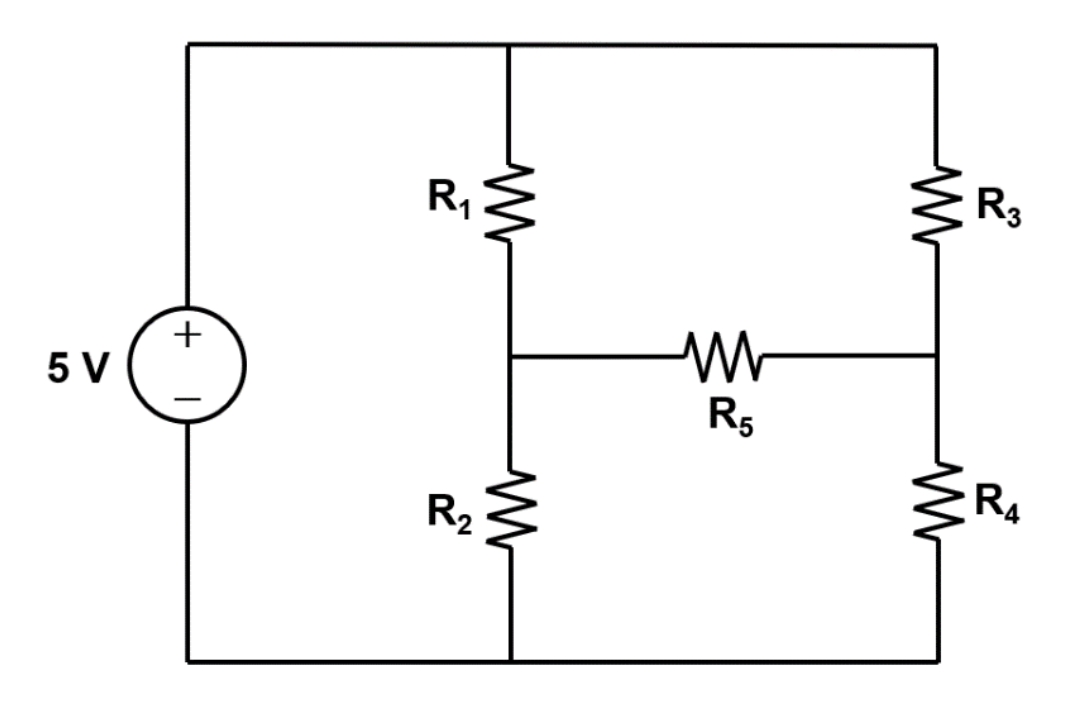
\includegraphics[width=0.5\textwidth]{images/setup.png}}\label{fig:setup2}
\subfigure[Breadboard Used]{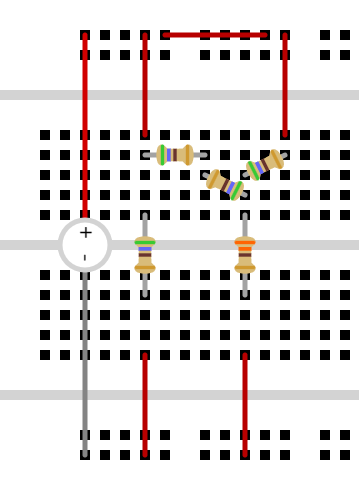
\includegraphics[width=0.25\textwidth]{images/breadboard.png}}\label{fig:breadboard2}

\caption{Set-Up Planned} \label{fig:2}
\end{figure}

In this experiment, to utilise a Breadboard to its best usage under this system, we have designed it as shown in Figure \ref{fig:2}. \\

We use nodal analysis to determine the relevant equations. We note that we denote $I_n$ as the current flowing through the resistor $R_n$.

\begin{figure}[h!]
    \centering
    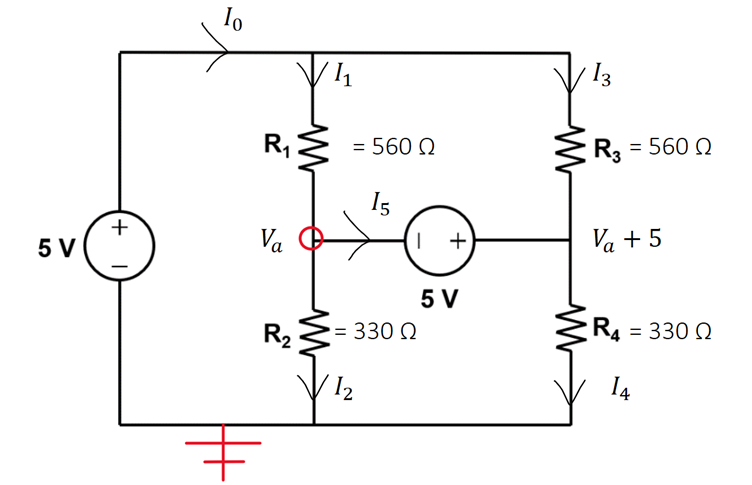
\includegraphics[width=\textwidth]{images/nodalAnalysis2.png}
    \caption{Nodal Analysis performed in the setup.}
    \label{fig:nodal2}
\end{figure}


To imagine the supernode, we go by the following expression:

\begin{align}
    \frac{5-V_a}{R_1} + \frac{5-V_a-5.08}{R_3} + \frac{0-V_a}{R_2} + \frac{0-V_a-5}{R_4} = 0
\end{align}

Essentially, we have imagined the strand containing the 5.08 V supply as the node.

We can simply said equation as follows:
\begin{align*}
    \frac{5-V_a}{R_1} + \frac{5-V_a-5.08}{R_3} + \frac{0-V_a}{R_2} &+ \frac{0-V_a-5}{R_4} = 0 \\
    \left(\frac{1}{R_1} + \frac{1}{R_3} + \frac{1}{R_2} + \frac{1}{R_4} \right) V_a &= \frac{5}{R_1} - \frac{0.08}{R_3} - \frac{5}{R_4}
\end{align*}

This gives us an expression for $V_a$, which can be computed as -0.747 V. Thus, we get the following cascade:

\begin{align*}
    I_1 &= \frac{5-V_a}{R_1} = 10.545\text{ mA} \\
    I_2 &= \frac{V_a}{R_2} = -1.368\text{ mA, which means current flows upwards} \\
    I_3 &= \frac{5-5.08-V_a}{R_3} = 1.215\text{ mA} \\
    I_4 &= \frac{5.08+V_a}{R_4} = 13.374\text{ mA}  \\
    I_5 &= I_4 - I_3 = 12.159\text{ mA}
\end{align*}

These can be plugged in as follows:

\begin{table}[!h]
    \centering
    \begin{tabular}{|P{15mm}|P{15mm}|P{15mm}|P{15mm}|P{15mm}|P{15mm}|P{15mm}|}
        \hline Resistor & Nominal \newline Resistance ($\Omega$) & Measured \newline Resistance ($\Omega$) & Calculated Voltage (V) & Calculated \newline Current (mA) & Measured \newline Voltage (V) & Measured \newline Current (A) \\
        \hline R_1 & 560 & 545 & 5.747 & 10.545 & 5.64 & 10.349 \\
        \hline R_2 & 560 & 546 & -0.747 & -1.368 & -0.79 & -1.447 \\
        \hline R_3 & 560 & 549 & 0.667 & 1.215 & 0.72 & 1.311 \\
        \hline R_4 & 330 & 324 & 4.333 & 13.374 & 4.83 & 14.907 \\
        \hline Second 5V Source & -- & -- & & 12.159 & -5.08 & 11.12 \\
        \hline
    \end{tabular}
    \caption{Table of Final Values}
    \label{tab:final2}
\end{table}

Now, notably, since the current flowing through the 5.08 V supply is flowing into the negative terminal and out of the positive terminal, we have that the supply is supplying power.

\end{document}
